%---DOCUMENT-------------------------------------------------------------------

\documentclass[a4paper,12pt]{report}
\usepackage[french]{babel}
\usepackage[utf8]{inputenc}
\usepackage[T1]{fontenc}
\usepackage{listings}

%---PACKAGES-------------------------------------------------------------------

\usepackage{makeidx} \makeindex
\usepackage[Rejne]{fncychap}				% Lenny, Conny ,Bjarne, Rejne, Glenn, Sonny
\usepackage{fancyhdr}
\usepackage{eurosym}
\usepackage{lastpage}
\usepackage{a4wide}
\usepackage[french]{minitoc}
\usepackage[hmargin=3.5cm,vmargin=2cm]{geometry}

%---SORTIES--------------------------------------------------------------------

\newif\ifpdf

\ifx\pdfoutput\undefined
   \pdffalse
\else
   \ifnum\pdfoutput=0
      \pdffalse
   \else
      \pdfoutput=1 \pdftrue
   \fi
\fi


%---PDF------------------------------------------------------------------------

\ifpdf
\usepackage[pdftex]{graphicx, color}
\graphicspath{{images/}}
\DeclareGraphicsExtensions{.jpg,.png,.gif,.bmp}
\pdfcompresslevel=9

\usepackage[pdftex, 					% Paramétrage de la navigation
bookmarks = true, 						% Signets
bookmarksnumbered = true, 		% Signets numérotés
pdfpagemode = None, 					% None, UseThumbs, UseOutlines, Fullscreen
pdfstartview = FitH, 					% FitH, FitV, FitR, FitB, FitBH, FitBV, Fit
pdfpagelayout = OneColumn, 		% SinglePage, OneColumn, TwoColumnLeft, TwoColumnRight
colorlinks = false, 					% Liens en couleur
urlcolor = black, 						% Couleur des liens externes
pdfborder = {0 0 0} 					% Style de bordure : ici, rien
]{hyperref}

\hypersetup{
pdfauthor = {\textsc{Huge Software}\\ Thomas A\"it-Taleb, Dimitri Georgoulis, Pierre Guilbert et Alexandre Testu}, 							% Auteurs
pdftitle = {Rapport de soutenance}, 								% Titre du document
pdfsubject = {Soutenance Finale}, 							% Sujet
pdfkeywords = {}, 						% Mots-clefs
pdfcreator = {}, 							% Logiciel qui a crée le document
pdfproducer = {} 							% Société avec produit le logiciel
plainpages = false}
\usepackage{pdfpages}

%---DVI------------------------------------------------------------------------

\else
\usepackage{graphicx}
\graphicspath{{eps/}}
\newcommand{\url}[1]{\emph{#1}}
\newcommand{\href}[2]{\emph{#2}[1]}
\fi

%---EN-TETE-ET-PIED-DE-PAGE----------------------------------------------------

\renewcommand{\headrulewidth}{0.5pt}
\renewcommand{\footrulewidth}{0.5pt}
\pagestyle{fancy}

%\lhead{}
%\chead{}
%\rhead{}
%\lfoot{}
%\cfoot{}
%\rfoot{}

%---PAGE-DE-GARDE--------------------------------------------------------------

\title{\textsc{Rapport de Soutenance} \\ Soutenance Finale}
\author{\textsc{Huge Software}\\ \\ Thomas A\"it-Taleb \\ Dimitri Georgoulis \\ Pierre Guilbert \\ Alexandre Testu}
\date{}

%---COLOR---------------------------------------------------------------------

%\pagecolor{}
% \color{}

%---DEBUT-DU-DOCUMENT----------------------------------------------------------



\begin{document}
\lstset{language=C}
\dominitoc
\maketitle
\tableofcontents \pagebreak
\thispagestyle{fancy}

\chapter{Introduction} % (fold)
\label{cha:introduction}

Ce document que vous avez en main est le rapport du projet ``OCRe'', le fruit de plusieurs mois de travail de quatre étudiants: Thomas Aït-taleb, Pierre Guilbert, Dimitri Georgoulis, et Alexandre Testu. \\
Vous tenez entre vos mains de nombreuses heures de stress, d’angoisse, de déceptions, mais aussi de joies, de découvertes, et surtout de camaraderie. Car OCRe est le fruit d’un travail d’équipe, d’une équipe aux membres très différents, mais qui, curieusement, tient debout. Oh, bien sûr, nous avons eu nos différends, tout le monde n’était pas toujours de bonne humeur, mais il y en avait toujours un pour redresser la situation et pousser les autres vers l’avant.

% chapter introduction (end)

\pagebreak

\section{Un OCR, what else?} % (fold)
\label{sec:un_ocr_what_else_}
Lorsque j’ai expliqué à ma mère le but de mon projet (``on doit réaliser un logiciel qui transformera une image en texte''), elle n’a pas compris. Je lui ai ré-expliqué en lui disant que l’on entrera du texte scanné, une image donc, et que notre logiciel reconnaîtra ce texte. Elle n’a toujours pas compris, et aujourd’hui encore ne comprend pas l’intérêt de notre application – il est utile de préciser que ma mère ne sait pas se servir d’un répondeur, mais qu’elle fait le meilleur coq au vin du monde. \\
Au fil du temps, je me suis rendu compte que ce n’était pas seulement ma mère qui ne comprenait pas, mais tout les gens qui n’utilisent pas régulièrement un ordinateur. Ils sont resté dans une logique d’\emph{impression}. L’ordinateur n’est pour eux qu’un lieu de passage pour leurs documents. Ces documents n’existent pas \emph{vraiment} s’ils ne sont pas sur du papier. \\
Or dans le monde dans le quel nous vivons et dans lequel nous \emph{vivrons}, le papier a de moins en moins d’importance. Nous souhaitons sa mort, et ce le plus rapidement possible. C’est pour ça que nous avons choisis ce projet, c’est parce que nous souhaitons développer une application réellement utile, voire indispensable. \\
Notre application est une machine à tuer le papier, elle extrait l’âme du papier – son contenu – pour nous permettre de le brûler avec un rictus machiavélique. \\

Plus sérieusement, nous croyons dur comme fer à la nécessité d’une telle application dans le monde d’aujourd’hui, alors qu’une application qui transforme des cartes 2D en modèles 3D, c’est certes \emph{cool}, mais ça s’arrête là. Nous croyons surtout que l’OCR peut être – et doit être – une application qui puisse être utiliser par \emph{tout le monde}. Tout le monde devrait pouvoir enregistrer facilement leurs documents papier sur leur ordinateur. Tout le monde devrait pouvoir, en un seul clic, obtenir le texte contenu dans un document scanné. C’est donc dans cette optique que nous avons choisi le projet de l’OCR, en souhaitant réaliser non pas une application compliquée, pleine d’options, mais un logiciel simplissime, qui n’ait qu’une seule fonction, mais qui la remplisse correctement.
% section un_ocr_what_else_ (end)


%%debut chapitre sur le programme ocred
\chapter{ OCRed, k\'ezako ? }
 OCRed est n\'e des mots Ocre et digital, qui rappellons le encore une fois
 signifient ``Optical Character Recognition enhanced'' pour l'un et
 num\'erique pour l'autre. La partie du projet portant sur le
 pr\'etraitement de l'image devant \^etre faite en ocaml, OCRed est
 totalement r\'ealis\'e dans ce langage.

\section{ Visualisation de l'image grace a l'executable }
 La cr\'eation du logiciel de traitement de l'image nous a men\'e, au
 d\'ebut du projet \'a vouloir visualiser directement, c'est \'a dire
 sans logiciel tiers, l'action de notre travail.
 La visualisation des images trait\'ees permet notre ind\'ependance
 au niveau de l'utilisation du logiciel, ce qui est un confort certain.
 La fen\^etre est r\'ealis\'ee avec OcamlSDL, tout comme le pr\'etraitement
 de l'image.
%% mettre image de la fenetre sdl

\begin{center}
	
	\includegraphics[width=70mm]{visualisationimage.jpg}\\
\end{center}

\section{Utilisation}
 L'ex\'ecutable en ligne de commande admet un certain nombre d'arguments,
 certains ne pouvant \'evidemment donner lieu \`a un quelconque r\'esultat
 sans la sp\'ecification d'une image d'entr\'ee.
\subsection{ Sp\'ecifier une image d'entr\'ee }
 Il est plus logique, pour un logiciel de traitement d'image, d'avoir
 une image \`a traiter. Vous devez pour cela utiliser l'argument ``-i''
 suivi du chemin d'une image de type jpeg,bmp,png au moins.
\subsection{ Sp\'ecifier une image de sortie }
 Vous n'\^etes pas oblig\'e de pr\'eciser le chemin de l'image de sortie
 mais cela permet une certaine flexibilit\'e. Dans le cas o\`u vous
 n'indiquez pas la sortie, OCRed se debrouille pour sortir une image
 avec un nom assez \'evident, d\'ependant du traitement. Par exemple
 rotatation.bmp ou encore tresholded.bmp, les images se trouveront l\`a
 o\`u vous avez ex\'ecut\'e votre programme. Pour sp\'ecifier un chemin de
 sortie, veuillez utiliser l'argument ``-o'' suivi du chemin d'une image
de type jpeg,bmp,png au moins.
\subsection{ La visualisation de l'image }
 Gr\^ace \`a OcamlSDL, nous pouvons visualiser notre image, il faut pour
 cela sp\'ecifier une image d'entr\'ee, et passer l'argument ``-d'' en
 param\`etre. Les d\'esavantages de l'utilisation de cette interface sont
 assez subtils, par exemple vous ne pouvez ni zoomer ni d\'ezoomer, ni
 vous d\'eplacer sur l'image. Toutefois il y'a (aussi) des avantages, vous pouvez
 visualiser directement les modifications appliqu\'ees \`a votre
 image. En appuyant sur F2 vous faites tourner l'image de l'angle que
 vous avez pass\'e en param\`etre --voir plus loin--. En appuyant sur F3
 vous appliquez le seuil, que vous pouvez sp\'ecifier en ligne de
 commande. En appuyant sur F4, vous appliquez le filtre m\'edian. Nous
 tenons \`a vous rappeler que le seuil ne marche que sur les couleurs.
 Pour quitter il suffit d'appuyer sur F1, la petite croix en haut \`a
 droite ne marche pas.
\subsection{ Le seuil }
 Permet le passage d'une image en noir et blanc, pour avoir un minimum
 de pertes d'informations vous devez sp\'ecifier un seuil viable. Par
 d\'efaut le seuil est \`a 200, ce qui est suffisant pour un contraste
 normal de l'image. Vous devrez l'augmenter si il est trop faible et le
 baisser dans le cas contraire. Passer l'argument ``-s'' en
 param\`etre si vous voulez changer la valeur par d\'efaut. Pour
 l'anecdote ``-s'' viendrait de seuil, mais nous n'en sommes pas vraiment
 s\^urs.
\subsection{ Rotation }
 Vous pouvez passer un angle en pr\'ecision r\'eelle, ou enti\`ere. Pour
 cela passez respectivement l'angle avec l'argument ``-af'' et ``-a''.
 Rappelons que l'angle pass\'e en param\`etre est en degr\'es et non en
 radian. Vous pouvez aussi tourner l'image de 90 degr\'es dans le sens
 direct ou indirect, gr\^ace aux options ``-right'' et ``-left''.
\subsection{ Redimensionnement }
 Le redimensionnement peut s'effectuer en pourcentage de l'image avec
 l'option ``--resizepercent'' qui prend en param\`etre un pourcentage
 entier. L'on peut aussi redimensionner l'image en valeur absolue
 --c'est \`a dire en sp\'ecifiant des valeurs de hauteur et de largeur
 arbitraires--. Alexandre Testu avait besoin d'un petit redimensionnement
 rien que pour lui, c'est pour cela que l'option ``--resize-auto''
 existe.
\subsection{ D\'etection d'angle}
 Il existe un argument magique ``-dev'' qui a juste besoin d'avoir une
 image qui n'est pas bien droite en param\`etre. Il retourne directement
 l'image dans le bon sens, et en noir et blanc.
\subsection{ Help me if you can! }
 L'option ``-help'' est aussi pr\'esente afin d'accompagner
 l'utilisateur dans sa d\'ecouverte du programme. Pour tout autre
 interrogation, il se peut que vous puissiez trouver des informations
 plus ou moins utiles dans les sources du projet, au niveau du fichier
 README.
%%fin chapitre sur le programme ocred


%%debut chapitre detection de l'angle
\chapter{D\'etection de l'angle }
 La d\'etection de l'angle \'etait \`a faire pour la premi\`ere
 soutenance, malheureusement par un manque de temps certain elle ne f\^ut
 pas pr\^ete \`a temps. Nous arrivons \`a la deuxi\`eme soutenance avec
 deux types de d\'etection de l'angle de rotation du texte d'une image,
 ce qui a pour but de redresser l'image, afin d'avoir une segmentation
 \`a peu pr\`es correcte.

\section{ Diff\'erentes approches}
 La d\'etection de l'angle de rotation d'un texte dans une image est un
 probl\`eme assez complexe. En effet une image contenant du texte n'est
 pas compos\'ee de composantes continues, il est donc plus difficile d'isoler
 les caract\'eristiques des \'el\'ements. Deux principes majeurs nous
 sont apparus. Tout d'abord l'on \'etudie les caract\'eristiques d'une
 image pour chaque angle, on isole ensuite le bon angle ; ce
 processus est long et d'autre part encore assez impr\'ecis.
 L'autre principe \'etait de d\'etecter la pente d'une ligne de caract\`eres.
\subsection{ La multiple rotation }
 Dans cet algorithme, l'on reduit la taille de l'image pour gagner en
 temps d'ex\'ecution, le redimensionnement est calcul\'e en fonction de la
 taille d'origine de l'image, on suppose avoir du format A4 \`a chaque
 fois. On proc\`ede comme suit: On tourne de fa\c con dichotomique
 l'image, c'est \`a dire en prenant des angles plus ou moins
 grand. Jusqu'a trouv\'e un histogramme convenable. L'histogramme est
 produit \`a partir de la projection de tout les pixels de l'image sur
 l'axe des horizontales.

Preuve exp\'erimentale produite \`a partir d' une image multifontes,
multicouleurs, mulicolonnes:

 Comme vous pouvez le voir sur ces images, il est \'evident qu'il y'a une
 nette diff\'erence entre des images avec un texte mal orient\'e et un
 texte orthonormal. (mais o\`u est l'orthonormalit\'e dans ce monde ?)

%% histogramme5degree.jpg
%% commentaire de l'image

\begin{center}
	
	\includegraphics[width=120mm]{histogramme5degre.jpg}\\
\end{center}


Sur cette image on peut voir un histogramme d'une image avec un
texte ayant subi une rotation de 5 degr\'es. Il est clair que le nombre
de zone ou l'histogramme atteint 0 en ordonn\'ee est beaucoup plus faible
que les autres images (environ 8).


%% rotation1deghisto.jpg
%% commentaire de l'image
\begin{center}
	
	\includegraphics[width=120mm]{rotation1deghisto.jpg}\\
\end{center}

Sur cette image on peut voir un histogramme d'une image avec un texte
ayant subi une rotation de 1 degr\'e. Par rapport \`a l'image
pr\'ec\'edente, on voit de fa\c con \'evidente que le nombre d'ordonn\'ees
\`a z\'ero est bien plus grand avec un angle de un degr\'e (ici environ 18).

%% histogramme_bon.jpg
%% commentaire de l'image

\begin{center}
	
	\includegraphics[width=120mm]{histogramme_bon.jpg}\\
\end{center}

Sur cette image on peut voir un histogramme d'une image avec un texte
n'ayant pas subi de rotation. Il est tr\'es net que le nombre
d'ordonn\'ees \`a z\'ero est le plus \'elev\'e.

Il est facile d'implementer un algo qui compte le nombre de bandes
proche de z\'ero ; il s'av\`ere que nous avons voulu compter le nombre de
sommets, ce qui est beaucoup moins pr\'ecis. La m\'ethode expos\'ee
ci-dessus semble bien marcher en th\'eorie.

\subsection{ Detection de la pente }
On d\'etecte la pente d'une ligne de texte ; pour cela on parcourt
l'image pour chaque ligne de pixels jusqu'\`a ce que l'on tombe sur un
pixel noir. Ceci permet d'avoir une certaine id\'ee de la pente d'une ligne
de texte. La tangente de cette pente nous donne l'angle par rapport \`a
la verticale. On la soustrait \`a 90 degr\'es si elle est positive, on
l'ajoute sinon. On se retrouve avec un angle qui correspond, avec un
taux d'erreur proche du dixi\'eme de degr\'e d'angle.

% mettre l'image histo_pente.jpg
% commentaire image histo_pente

\begin{center}
	
	\includegraphics[width=120mm]{histo_pente.jpg}\\
\end{center}

Les extrema locaux de la courbe sont beaucoup moins \'elev\'es en
terme de valeurs. Ce qui a pour cons\'equence, une pente peu \'elev\'ee et donc un angle tr\`es \'elev\'e.

% mettre l'image histo_pent_noangle.jpg
% commentaire image histo_pent_noangle


\begin{center}
	
	\includegraphics[width=120mm]{histo_pente_noangle.jpg}\\
\end{center}

Les extrema locaux de la courbe sont beaucoup plus \'elev\'es en
terme de valeurs que ceux de la courbe pr\'ec\'edente. Ce qui a pour
cons\'equence, une pente tres \'elev\'ee et donc un angle tr\'es faible.

Le probl\`eme avec cette technique, et le manque de pr\'ecision autour
de l'angle nul, et des bruits trop importants produits par des lignes,
tableaux, ou images impromptus.

Nous avons pourtant retenu cette technique pour cette soutenance, car
donnant lieu \`a des r\'esultats plus probants que la m\'ethode expos\'ee
plus haut.

\section{ Optimisations  }
 L'optimisation est un crit\`ere de confort pour l'utilisateur, mais
 surtout un gage de qualit\'e.
\subsection{ R\'eduction de l'image }
 Afin de pouvoir augmenter la rapidit\'e des algorithmes de d\'etection
 d'angle, nous r\'eduisons l'image de sorte qu'il y ait le moins de
 pertes d'informations n\'ecessaires \`a cette derni\`ere. A titre
 d'exemple une image au format A4 en 75 dpi, a une taille approximative
 de 900 par 700. Les caract\`eres pr\'esents dans cette image ont une
 taille en pixels d'\`a peu pr\`es 8 pixels. Il ne faut donc pas trop
 r\'eduire l'image, environ 40 pourcents de la taille originale. Au
 contraire pour une image de plus haute d\'efinition, par exemple 600
 dpi, il est n\'ecessaire de r\'eduire l'image \`a au moins 5 pourcents
 de la taille originale. Et comme dirait Junior, ``l'id\'ee c'est
 que'' la rotation d'une image r\'eduite \`a 5 pourcents prend environ
 0,05 secondes sur les machines du PIE, alors qu'elle prend plus de 30
 secondes pour une image en 600 dpi.

%% reduceimage20percent75dpit.jpg
\begin{center}
	
	\includegraphics[width=40mm]{reduceimage20percent75dpit.jpg}\\
	\caption{\emph{Une image r\'eduite.}}
\end{center}
 

\begin{description}
	\item[Remarque:] Il est int\'eressant de noter qu'une image r\'eduite comporte
	moins de bruit, qui fausserait l'avanc\'ee de l'algo de reconnaissance
	des plages nulles.
\end{description}

\subsection{ Ce que nous aurions du faire}
\subsubsection{ D\'etection d'angle}
Notre d\'etection de l'angle de rotation d'un texte dans une image est
encore assez impr\'ecise ; cela est principalement d\^u \`a l'utilisation
de l'arctangente qui devient tr\`es sensible aux extrema. Nous pensons
donc r\'eutiliser la technique de la multiple rotation, qui semble en
th\'eorie plus pr\'ecise.
\subsubsection{ Optimisation des filtres}
Le gros probl\`eme de la rotation est la perte d'information, en effet
cette transformation a en sortie des nombres \`a virgule flottante,
ce qui ne correspond pas vraiment aux nombres entiers d\'efinissant la
grille d'une image dans le cas de pixels carr\'es. Une multitude de
filtres existent, mais le plus rapide et le plus adapt\'e dans le cas de la
rotation serait un filtre bicubique.
%%vive le copier coller a remanier en trente secondes:D
\Chapter{Utilisation de OCRed dans OCRe}
\section{Pourquoi?}
Notre programme, est cr\'ee dans l'optique d'une utilisation par un
consomateur lambda, dans cette optique, nous avons du cr\'eer diff\'erents
outils, qui communiquant entre eux, forment un tout unique et
merveilleux, OCRe.
OCRed \`a \'et\'e battit dans l'objectif de faciliter de le
pr\'etraitement, tache tr\'es difficile r\'ealis\'e par le programme segmentation.





\chapter{Analyse et extraction}

\section{Rappel des faits}

La partie analyse et extraction a pour but, comme son nom l'indique, d'analyser la
structure du document et d'extraire les caractères afin de pouvoir les communiquer à la
partie reconnaissance des caractères. Durant les deux premières soutenances, nous vous
avons présenté plusieurs principes de détection. Lors de la première soutenance, nous nous
sommes attachés à détecter les lignes en utilisant la méthode des projections de pixels.
Durant la deuxième soutenance, nous vous avons présenté la détection des
caractères. Celle-ci faisait appel à une méthode de segmentation par croissance de régions.
Cependant, à ce stade notre algorithme était seulement capable de récupérer les
composantes connexes, constituant ainsi les caractères. Pour les besoins de l'OCR, il
devenait impératif de regrouper l'ensemble de ces caractères en blocs. Ces mêmes blocs
nous renseigneraient ainsi sur la structure du document analysé. Pour réaliser cette
détection des blocs, nous avons donc continué sur notre voie en appliquant la fameuse
croissance des régions.

\begin{center}
  \includegraphics[width=130mm]{screenshot.jpg}
  \caption{\emph{Extrait d'un document segment\'e}}
\end{center}



\section{Principe de la segmentation}

La méthode de segmentation que nous avons utilisée pour cette soutenance est la suite
de celle là même utilisée lors de la dernière soutenance. C'est la méthode par segmentation
de régions (region-based segmentation), plus précis\'ement par croissance de régions
(growing-region segmentation). Elle est composée de deux étapes principales que l'on peut
associer respectivement au travail réalisé lors des deux dernières soutenances:

\begin{enumerate}
\item Trouver les points de départ de nos régions.
\item Faire grossir nos régions par agglomération des pixels voisins.
\end{enumerate}

La première étape, réalisée lors de la 2ème soutenance, consiste donc à trouver les
composantes connexes qui constitueront les points de départ de nos régions. Nous ne
détaillerons pas ici le principe de cette étape qui a déjà été abordée dans le rapport de la
2ème soutenance.

Nous nous intéressons ici à la deuxième étape de la segmentation, qui consiste à faire
croître nos régions par agglomération des composantes connexes entre elles. Nous
travaillons ici sur les composantes connexes qui nous sont fournies par la 1ère étape sous
forme d'une liste triée en ordre croissant de composantes connexes. Pour la suite du
rapport et la clarté de l'explication, les composantes connexes seront
assimilés aux caractères.

\begin{center}
  \includegraphics[width=90mm]{croissance.jpg}
  \caption{\\\emph{Explication du principe de segmentation par croissance de r\'egions}}
\end{center}



\section{Hierarchie des informations}

Pour implémenter cette deuxième étape de l'algorithme de segmentation par régions,
nous avons fait appel à de nouvelles structures de données. Celles-ci nous permettent
ainsi de représenter des mots, des lignes et des blocs de texte, que nous appellerons plus
communément des paragraphes. Ces nouvelles structures de données s'ajoutent à la
structure de composantes connexes qui est la structure atomique employée par
l'algorithme. En effet, dans notre cas, on ne peut pas décomposer des composantes
connexes, ce sont nos points de départs et les paragraphes seront ceux d'arrivée. Ces
différentes structures de données sont à employer selon une hiérarchie bien précise. Les
caractères (composantes connexes) constituent des mots, qui composent des lignes, qui
créent des paragraphes.

Afin de représenter ces données en mémoire, nous avons principalement repris la
structure des composantes connexes en la modifiant selon nos besoins. Nos données seront
donc stockées en mémoire grâce à des listes chaînées triées de caractères, de mots, de
lignes et de paragraphes. Voici les quatre types principaux nous permettant de représenter
les différents éléments cités ci-dessus:

\begin{lstlisting}
struct s_cc_elt
{
    int id;
    int nbpix;
    struct s_box_coordinate coord;
    int chr;
    struct s_cc_elt *next;
}

struct s_word_elt
{
    struct s_cc_list *cclist;
    struct s_box_coordinate coord;
    struct s_word_elt *next;
}

struct s_line_elt
{
    struct s_word_list *wordlist;
    struct s_box_coordinate coord;
    struct s_line_elt *next;
}

struct s_paragraph_elt
{
    struct s_line_list *linelist;
    struct s_box_coordinate coord;
  struct s_paragraph_elt *next;
}
\end{lstlisting}


Voici la hiérarchie des types de données utilisés. Vous pouvez constater qu'ils sont
similaires dans leurs structures. Ainsi, un paragraphe est constitué de ses propres
coordonnées et de la liste de lignes le composant. Cette même liste de lignes est composée
de ses coordonnées et de la liste des mots qui la composent. Et enfin cette liste de mots
possède ses propres coordonnées et la liste des caractères qui le composent. L'algorithme
d'agglomération des éléments devra parcourir l'ensemble des caractères pour
créer ainsi une liste de mots qui sera elle-même parcourues pour fournir une liste de lignes
et ainsi de suite jusqu'à obtenir la liste des blocs de texte: les paragraphes.

\begin{center}
  \includegraphics[width=90mm]{hierarchie.jpg}
  \caption{\\\emph{Hi\'erarchie des informations}}
\end{center}



\section{Impl\'ementation}

La première phase de la segmentation, à savoir la recherche des composantes connexes
est effectuée par la fonction findCC(), comme explicitée dans le précédant rapport. Cette
fonction nous renvoie une liste triée de composantes connexes. Cette liste constitue le
départ de la deuxième phase de la segmentation. La phase de croissance des régions se
réalise en trois étapes effectuées par trois fonctions principales dont voici les prototypes:

\begin{lstlisting}
t_word_list *makeWords(t_cc_list *cc_list);

t_line_list *makeLines(t_word_list *word_list);

t_paragraph_list *makeParagraphs(t_line_list *line_list);
\end{lstlisting}

Ces trois fonctions créent séquentiellement une liste de mots puis une liste de lignes et
enfin une liste de paragraphes. Voyons plus en détails leur fonctionnement respectif.
   
La fonction makeWords() prend en paramètre une liste de composantes connexes et
renvoie la liste des mots qu'elle a formés. Cette fonction parcourt la liste des composantes
connexes. Au premier caractère trouvé, elle crée un mot auquel elle associe une liste de
caractères. Tant que les caractères suivants respectent un seuil vertical et un seuil
horizontal spécifique alors on ajoute ces caractères au mot précédemment créé sinon on en
crée un autre. Le seuil vertical permet d'éviter d'ajouter des caractères provenant d'une
autre ligne et le seuil horizontal permet d'éviter d'ajouter des caractères trop espacés qui
feraient partis d'un autre mot.

\begin{center}
  \includegraphics[width=100mm]{seuils.jpg}
  \caption{\\\emph{Pr\'esentation des seuils horizontal et vertical}}
\end{center}

Selon le même modèle, la fonction makeLines() prend en paramètre une liste de mots et
renvoie une liste de lignes qu'elle a constituées. Cette fonction parcourt la liste des mots. Au
premier mot trouvé, elle crée une ligne et lui associe une liste de mots la composant. Elle
détecte les mots qui sont sur la même ligne grâce à un seuil vertical selon le même principe
que le seuil vertical de la fonction makeWords(). La fonction makeParagraphs() fonctionne
sur le même principe que les précédentes fonctions à ceci près qu'elle se situe à un niveau
supérieur dans la hiérarchie des données.



\section{Standardisation}

Une fois l'image segment\'ee, on se doit de stocker les informations obtenues pour que l'on puisse
les analyser ult\'erieurement. C'est pourquoi nous avons commenc\'e \`a d\'evelopper un module
permettant de sauvegarder aussi bien la structure lin\'eaire du document, \`a savoir la mise en page,
que les donn\'ees, ici les matrices de pixels correspondant aux caract\`eres. Nous avons donc \'et\'e
amen\'e \`a concevoir une fonction permettant de r\'ecup\'erer la matrice binaire d'\`apr\`es les coordonn\'ees
des \'el\'ements (composantes connexes, mots, lignes, paragraphes) ainsi que des fonctions nous permettant de
cr\'eer un fichier de type xml (travail r\'ealis\'e par Alexandre) contenant la hi\'erarchie des \'el\'ements
de la page ainsi que les coordonn\'ees des caract\`eres dans l'image du document. Cependant, un probl\`eme est
survenu. On se devait de standardiser les informations obtenues en matrices de 10 par 10 pixels pour l'entr\'ee
du r\'eseau de neurones, \`a savoir de redimensionner les matrices de pixels.
Or le retard accumul\'e ne nous a pas permis de finir cette \'etape de standardisation.


\section{Bilan}

Au terme du projet, la partie Analyse et extraction permet conformément au cahier des
charges de décomposer une image prétraitée qualifiée de ``parfaite'' en lettres, mots, lignes
et paragraphes. On constate cependant des imprécisions dans les blocs détectés. Elle
permet en outre de stocker en mémoire la structure linéaire du document ainsi que les
données textuelles. Cependant, le retard que nous avons accumulé depuis la dernière
soutenance ne nous a pas permis de terminer l'étape de standardisation des données pour
le réseau de neurones.








%% merde
%% debut du chapitre sur les reseaux de neuronnes
\chapter{ R\'eseau de Neurones Formels?}
%%mettre ca en jolie pour TESTU

\section{ Qu'est-ce qu'un RNF?}
Un RNF est un r\'eseau de neurones form\'els, bon jusque l\'a vous me
suivez, quoique pas sur. On va essayer d'y remedier.
\subsection{Historique}
Le domaine des r\'eseaux de neurones, dont les traditions sont
anciennes, a \'et\'e saisi par une p\'eriode d'effervescence
the\'eorique et interdisciplianire pendant les ann\'ees quatre-vingt,
suivie par une phase d'explorations tous azimuts au cours de la
d\'ecennie suivant. Ca c'est pour l'introduction.
Pendant les ann\'ees 1980, les travaux et recherches sur les neurones
formels rassemblaient une multitude de chercheurs venant d'horizons
tout aussi divers que la physique statistique, la biologie,
la psychologie et l'ing\'enierie, qui esp\'erer profiter de cette
situation.

Collaborations entre biologistes et physiciens se sont prolong\'e
surtout sur des probl\`emes th\'eoriques dans les ann\'ees 90. A cette
m\'eme \'epoque, les ing\'enieurs ont d'ailleurs commenc\'es la
r\'ealisation gr\^ace aux rnfs, de syst\'emes fonctionnels en
reconnaissance de formes et en mod\'elisation non-lin\'eaire.
Ces derni\`eres avanc\'ees sont notamment du aux r\'esultats
math\'ematiques et statistiques importants qui on vu le jour en ce
d\'ebut de d\'ecennie(1990 j'entends). De plus la
recherches dans ce domaine, qui n'a pas cess\'e, a apport\'e de nombreuses solutions
d'optimisation ces derni\'eres ann\'ees, principalement pour les
prob\'emes d'estimations des param\'etres du reseaux, et des
m\'ethodes d'\'evaluation de la qualit\'e d'un classifieur.

Rappelons, qu'au d\'epart l'on a appell\'e cela par analogie avec les
syst\'emes biologiques, car oui nous sommes tous dot\'ees plus ou
moins d'un certain nombres de neurones. M\^eme moi.

Aujourd'hui principalement \'a cause de la nature statistiques des
r\'eseaux de neurones, cette analogie semble devenir d\'esu\`ete.
On pourrait m\^eme dire que les pseudo-justifications biologiques des
architectures et des algorithmes ne sont plus de mise, mais l\`a ce
n'est pas de moi.

Et l\`a normalement vous me dites, et avant les ann\'ees quatre-vingt
y'avait quoi? Bonne question: \dots d'apr\`es mes sources, une certaine
personne du nom de Marvin Minsky, connu pour ses th\'eories sur la
hierarchisation du syst\'eme de pens\'ees humain, mais aussi pour sa
d\'ecouverte de l'inutilit\'e du r\'eseau de neurones formels tels
qu'il \'etait envisag\'e dans les ann\'ees 70. Rummelhart introduit
alors le perceptrons multicouches en 1984, dont la grande nouveaut\'e
est la r\'etropropagation du gradient.

\subsection{Ca sert a quoi?}
Bon c'est bien beau tout \c ca mais a quoi  \c ca sert? On a
dej\'a effleur\'e le sujet dans l'historique, mais on va
approfondir. Les r\'eseaux de neurones formels servent
particuli\'erement \`a la mod\`elisation statique et dynamique, la
commande de processus, et la classification. Vous allez me dire
comment une simple structure de donn\'ees avec deux trois m\'ethodes
peut reconnaitre un objet, mod\`eliser un syst\`eme dynamique? C'est
ce que j'appelle une question.
Les rnfs dont il est question ici doivent etre considerees comme des familles de fonctions parametres
modulatoires et possedant de bonnes propriet\'ees
d'approxiamation. Pourquoi parceque leurs applications leur demande
d'etre ainsi.
De nombreux probl\`emes industriels o\' de recherche demandent de
repr\'esenter a l'aide dun mod\`ele math\'ematique le comportement de
processus physiques,chimiques,\'economoiques etc.. a partir de
connaissances sur ce comportement et de mesures effectu\'ees
sur le processus. Un tel mod\`ele peut etre construit pour :
analyser les phenomenes regissant le comportement du processus;
predire a court ou a long termes les grandeurs d'interet du processus
concevoir un systeme de commande du processus.
O\'u un processus est une entit\'e qui fournit un ou plusieurs
grandeurs qui nous interessent. cette grandeur peut etre n'importe
quoi, cela peut etre un debit, un
potentiel pour un processus de production une population ou encore
pour un processus biologique ou ecologique.., par exemple des poissons?
Generalement cette grandeur d'interet est la sortie de notre reseau de
neurones.

Bon en resume, on peut dire qu'un reseau de neurones ca sert
principalement a trois domaines, la classification ou la
reconnaissance de motifs, la modelisation de systeme biologique,
industrielle, mecanique, et la commande de processus ou automates pour
les intimes. Le principale avantage des reseaux de neuronnes par
rapport a des modeles dit de systeme statistiques, ou expert la
rapidite. Cela est principalement du a la faible quantite de calcule
pour l'utilisation  d'un reseau de neurones formels.
\subsection{Diff\'erent Mod\`ele}

Il existe de nombreux mod\'eles de reseaux de neurones formels, mais
bon principalement, comme on l'a expliqu\'e plus haut, c'est un
syt\`eme qui nous donne une sortie qui d\'epend d'entr\'ees externes
ou pas. Le premier mod\`ele qui nous vient \`a l'esprit est le
mod\`ele dit de ``boites noires'' , il y'a ensuite les mod\`eles dit
lin\'eaires et non-lin\'eaires et puis finalement le mod\`eles qui
d\'ependent du temps, de fa\c con discr\`ete ou continue. Sachant
qu'on peut m\'elanger raisonnablement ces diff\`erentes propri\'etees.
Un mod\`ele de type boite noire, peut-etre non-lin\'eaire par rapport
\`a ses param\'etres ou bien le contraire, le mod\`ele de la boite
noire s'utilise aussi bien pour \'etudier le comportement statiques
d'un transistor MOS en saturation, que le mod\'ele d'une r\'eaction
enzymatique par rapport \`a son substrat.

Les rnfs sont des familles de fonctions non lineaire modulaires
capables d'approximer n'importe quelle fonction bornee dans un
interval bornees de ses entrees aussi complexe soit-elle. C'est l'une
des raison pour lesquelles le rnfs sont utilises comme modeles
boite-noire non lineaire statiques(reseau non boucle, donc sans
retroaction)..et mod\`ele dit dynamique(reseau boucle, avec
retroaction). La mise au point d'un modele neuronal consiste a
calculer ses parametres de telle sorte que la sortie du modele predise
celle du processus en moyenne . en termes statistiques on desire
estimer les parametres de telle facon que la sortie du modele soit
aussi proche que possible de l'espereance mathematique de la sorite
du processsus . Cette esperance mathematique qui est une fonction
inconnue des entrees est appelle la regression. l'estimation de
ces parametres appele apprentissage dans la communaute neuronale est
realis\'e  a l'aide d'un ensemble d'apprentissage constitu\'e de couples
de valeurs d'entres et de sorties appel\'e exemples d'apprentissage.

%% mettre plein d'images kikoo lol
\subsection{Exemple}
Par exemple un classifieur: on veut proceder a la classification de
chiffres decimaux manuscrits: les entrees prennent les valeurs - ou 1
selon celles de pixels de l'images binarise du chiffre presente. Les
classe d'appartencae sont {0 1 2 3 4 5 6 7 8 9}.
Un classifieur est ainsi pour attribuer un objet represente par
un vecteur d'entree a une classe d'appartencance. Par exemple dans le
cas d'un probleme a deux classe la sortie du classifieur est une
variable qui prend la valeur 1 pour la premiere classe et 0 pour la
deuxieme.
En gros, et pour faire simple on a une espece de representation des
entrees/sorties sur un plan en deux dimensions, on trace une
courbe.. et d'un cote on a la valeur de sortie a un, et de l'autre
cote on a la valeur de sortie a 0.

Et maintenant des images parce nous le valons bien:

%% mettre plein d'image kikkoo lol 2
%% tu les mets toutes la dedans et puis je te sors les commentaires
\begin{center}
	
	\includegraphics[width=40mm]{IMG_7234.JPG}\\
	\caption{\emph{Neurone Formel \`a potentiel.}}
\end{center}

\begin{center}
	
	\includegraphics[width=40mm]{IMG_7235.JPG}\\
	\caption{\emph{Repr\'esentation des entr\'ees sorties.}}
\end{center}

\begin{center}
	
	\includegraphics[width=40mm]{IMG_7236.JPG}\\
	\caption{\emph{Mod\`ele neuronal \`a une couche de neurones cach\'e.}}
\end{center}

\begin{center}
	
	\includegraphics[width=40mm]{IMG_7237.JPG}\\
	\caption{\emph{Rnfs pour sigmoides, avec un neurones de biais}}
\end{center}

\begin{center}
	
	\includegraphics[width=40mm]{IMG_7238.JPG}\\
	\caption{\emph{Un exemple de ce que nous n'avons pas fait}}
\end{center}

%% pour les images


%%% PARTIE DE DIMMII


\chapter{Notre r\'eseau de neurones} % (fold)
\label{cha:notre_reseau_de_neurones}

\section{Introduction} % (fold)
\label{subsec:introduction}
A l'issue de la premi\`ere soutenance, nos recherches sur les r\'eseaux
neuronaux nous avaient men\'es vers l'\'elaboration d'un perceptron
multicouches, celui-ci \'etant reconnu comme la star de la
reconnaissance de caract\`eres.

Le temps a pass\'e', \'ecrivait G\'erard de Narval, pensant \`a sa jeunesse
et toutes ces belles ann\'ees d\'esormais r\'evolues... En ce qui
concerne le r\'eseau de neurones, le temps a \'egalement pass\'e et
notre perceptron multicouches commence \`a prendre de l'allure. Sa
jeunesse n'\'etant pas encore r\'evolue, grand bien lui fasse, il a
encore beaucoup \`a apprendre... Alors
certes il ne reconna\^it pas encore grand chose, mais une premi\`ere
\'ebauche de sa structure est pr\^ete et les premiers tests ont \'et\'e
effectu\'es sur les donn\'ees d'un XOR et celles d'un afficheur sept
segments. La phase d'apprentissage reste \`a mettre au point car la
version actuelle ne donne pas les r\'esultats attendus. Mais ne parlons
pas de malheur, et rentrons d\`es \`a pr\'esent dans le vif du sujet : what about
multi-layer perceptron ?! 

Nous d\'ecrirons ici le perceptron tel que nous l'avons abord\'e, c'est \`a
dire \`a un stade encore exp\'erimental. Pour motiver sa conception,
nous nous sommes plac\'es dans le cas o\`u notre r\'eseau devra
reconna\^itre les caract\`eres provenant d'un afficheur sept
segments. En effet, les donn\'ees d'un tel alphabet sont assez simples
\`a formater sans pour autant atteindre le niveau de simplicit\'e d'une
fonction logique de base comme le OR ou l\'eg\`erement plus avanc\'ee
comme le XOR

% subsection introduction (end)
\pagebreak
\section{Structure et d\'efinitions} % (fold)
\label{subsec:structure_et_definitions}

Voici ce \`a quoi ressemble la b\^ete :
\begin{center}
	
	\includegraphics[width=120mm]{ra-perceptron.png}\\
	\caption{\emph{Perceptron \`a une couche cach\'ee}}\\
\end{center}

%pour ce paragraphe j'aimerais une liste à puce à la place de mes étoiles
%=)
Un perceptron est un ensemble de neurones reli\'es par des connexions
pond\'er\'ees. Ce n'est rien d'autre qu'un graphe non-orient\'e valu\'e
en somme, du moins en apparence. On y rep\`ere trois ensembles
particuliers de neurones que sont : 
%debut de liste à puce
\begin{itemize}
	\item la couche d'entr\'ee : elle poss\`ede un certain nombre de neurones qui
correspondent \`aux entr\'ees du r\'eseau. La mod\'elisation et le
formatage des donn\'ees d'entr\'ee sont donc primordiaux si l'on veut
\'eviter d'avoir un trop grand nombre de neurones, ce qui augmenterait
le temps de la reconnaissance par la suite.


\item la ou les couches cach\'ee(s) : ce sont ces neurones qui permettront de
reconna\^itre des donn\'ees. Le nombre de couches cach\'ees et de
neurones par couche est \`a adapter selon le probl\`eme et en
particulier selon la taille de l'\'echantillon de donn\'ees que l'on veut
apprendre au r\'eseau.


\item la couche de sortie : ce sont ces neurones qui contiendront le
r\'esultat de la reconnaissance. Il y en a, a priori, autant que
d'\'elements \`a reconna\^itre, mais une seule sortie ensuite filtr\'ee
par une table de hachage,par exemple, reste envisageable.


\end{itemize}
%fin de liste a puce

% Mettre cette photo ici !

\begin{center}
	
	\includegraphics[width=70mm]{sortie008.png}\\
	\caption{\emph{Perceptron \`a une sortie}}\\
\end{center}




% avec la légende suivante : Perceptron \`a une sortie

La valeur d'un neurone est calcul\'ee \`a partir des valeurs de chacun
des neurones de la couche pr\'ec\'edente.

Les neurones artificiels ainsi \'evoqu\'es sont en fait tr\`es proches
des neurones naturels au niveau de leur fonctionnement. C'est entre
autres l'id\'ee d'int\'eractions avec une multitude d'autres neurones
qui permet au r\'eseau de se constituer une ``m\'emoire intelligente'',
apte \`a classifier ou reconna\^itre des donn\'ees qu'il n'a encore
``jamais'' rencontr\'ees auparavant (du moins pas exactement sous la
même forme) !

Avant de pouvoir utiliser un perceptron multicouches, il faut avant tout se mettre d'accord sur le
format de donn\'ees qu'il prendra en entr\'ee, puis effectuer un choix
judicieux de son nombre de couches cach\'ees et de son nombre de neurones
par couche cach\'ee. On doit ensuite ``entra\^iner'' le r\'eseau\ldots

% subsection structure_et_definitions (end)

\section{Formatage des donn\'ees} % (fold)
\label{subsec:formatage_des_donnees}

Pour que le r\'eseau reconnaisse, dans notre cas, si un caract\`ere est
telle ou telle lettre, il faut affecter une valeur pr\'ecise à chacun de
ses neurones d'entr\'e.
Parmi les id\'ees qui nous sont venues, il y a l'extraction de
caract\'eristiques des caract\`eres que l'on a isol\'e \`a partir du document
scann\'e. Ainsi l'on pourrait envisager de vectoriser chaque caract\`ere
afin d'en extraire des segments caract\'eristiques que l'on donnerait en
entr\'ee au r\'eseau. On pourrait aussi imaginer effectuer une premi\`ere
classification par crit\`ere de largeur, puis de hauteur, etc, en utilisant
plusieurs r\'eseaux en s\'erie par exemple, jusqu'\`a d\'etermination totale du
caract\`ere.

La m\'ethode que nous avons retenue \`a ce jour est n\'eanmoins bien
plus simpliste, et pas n\'ecessairement moins efficace : notre
perceptron recevra directement la matrice de pixels associ\'ee au
caract\`ere \`a reconna\^itre, apr\`es calibrage et centrage de chaque
caract\`ere dans une matrice de taille fixe.
Chaque neurone d'entr\'ee du r\'eseau recevra donc l'un des pixels de la
matrice de caract\`ere (d'o\`u la n\'ecessit\'e de r\'eduire au maximum
la taille et l'\'epaisseur de nos caract\`eres, afin de ne pas
d\'epasser la centaine de neurones d'entr\'ee).
Les donn\'ees d'apprentissage seront quant \`a elles pr\'esent\'ees sous
forme de couples de vecteurs d'entr\'ees/sorties au r\'eseau et
stock\'ees dans un fichier.


% subsection formatage_des_donnees (end)

\section{Param\`etres du r\'eseau} % (fold)
\label{subsec:choix_des_parametres_du_reseau}

Une fois les donn\'ees format\'ees et stock\'ees dans un fichier, il
faut choisir un certain nombre d'éléments clés du réseau.

Nous avons donc choisi d'affecter chaque pixel de la matrice du
caract\`ere \`a reconna\^itre \`a un neurone d'entr\'ee.

Dans le mod\`ele retenu actuellement, nous pr\'evoyons aussi d'affecter
un neurone de sortie par caract\`ere \`a reconna\^itre. Le caract\`ere
reconnu sera celui dont la valeur sera \`a un alors que les autres seront
rest\'es \`a z\'ero.

Pour ce qui est des couches cach\'ees, il est recommand\'e dans le cas
de la reconnaissance de caract\`eres d'en prendre entre une et deux, et
de choisir un nombre de neurones par couche du m\^eme ordre de grandeur
que le nombre de neurones de la couche de sortie. Mais nous essayerons
plusieurs configurations jusqu'\`a obtenir des r\'esultats
performants.

Un certain nombres de param\`etres relatifs \`a l'apprentissage des
donn\'ees par le r\'eseau doivent \'egalement \^etre fix\'es. Nous en
ferons une br\`eve description dans la section ``Entra\^inement du r\'eseau.''

% subsection choix_des_parametres_du_reseau (end)

\section{Entra\^inement du r\'eseau} % (fold)
\label{subsec:entrainement_du_reseau}

Cette partie est tr\`es probablement la plus int\'eressante de
l'impl\'ementation du perceptron multicouches. C'est en effet ici que
l'on doit mettre en oeuvre le fonctionnement du r\'eseau \`a proprement
parler. 

Son principe est le suivant :

Dans un premier temps, on affecte des petites valeurs \`a tous les poids
des connexions neuronales (entre 0,5 et -0,5 dans notre cas).

Ensuite, pour un nombre d'it\'erations donn\'e par exemple, ou bien tant
que l'erreur totale du vecteur de sorties est supérieure à un seuil fixé, on effectue
les \'etapes suivantes :

On permute l'ordre des donn\'ees que l'on pr\'esente au r\'eseau, ceci
d'uniformiser l'apprentissage, de sorte \`a ce qu'il n'apprenne pas \`a reconna\^itre toujours la m\^eme
s\'equence de donn\'ees.

On fournit ensuite un couple d'entr\'ees/sorties d\'esir\'ees au
r\'eseau.

Il faut maintenant propager vers l'avant les valeurs des neurones
d'entr\'ee, de sorte \`a obtenir les valeurs de sortie.

Pour cela on utilise une fonction de combinaison, ici une somme
pond\'er\'ee sum, dans notre cas
d\'efinie comme, pour chaque neurone ni, la somme des produits des valeurs
des neurones nj qui pointent sur lui par les poids des connexions pij qui les
lient au neurone courant :

\[sum(ni) = somme\, sur\, j\, (pij(ni,nj)* valeur(nj))
\]% une formule en LaTeX serait plus jolie ici
\\

\begin{center}
	
	\includegraphics[width=70mm]{neuron.jpg}\\
	\caption{\emph{Calcul de la sortie d'un neurone}}\\
\end{center}




Cette valeur est ensuite pass\'ee en param\`etre d'une fonction
d'activation propre au perceptron, ici la fonction sigmo\"ide f avec :  

\[f(sum(ni)) = 1/(1+exp(-sum(ni))) 
\]% une formule en LaTeX serait plus jolie ici

On obtient ainsi une valeur exp\'erimentale pour chaque neurone de
sortie que l'on va pouvoir confronter \`a la valeur th\'eorique fournie
initialement.

On calcule donc l'erreur e observ\'ee pour chaque neurone de sortie ni avec :

\[
	e(ni) = (valeur\, theorique(ni)\, -\, valeur\, observee(ni))*(f'(sum(ni)))
\]

% une formule en LaTeX serait plus jolie ici

On propage ensuite l'erreur vers les couches intérieures 

Puis on modifie les poids de toutes les connexions du réseau.

Et voilà, notre réseau marche !! Du moins pour apprendre le XOR !! Car
nous avons hélas manqué de temps pour conclure ce merveilleux projet et
nous comptons bien sur les vacances d'été pour le recoder intégralement
!



% subsection entrainement_du_reseau (end)

\subsection{Le banc de tests du perceptron} % (fold)
\label{subsec:le_banc_de_tests_du_perceptron}

Un petit shell a \'et\'e impl\'ement\'e afin de tester notre perceptron
au fur et \`a mesure de sa cr\'eation. Il est lanc\'e par d\'efaut lors
de l'ex\'ecution du programme ``network'' et propose diverses
options. 
%une grosse liste à puce please !
\begin{itemize}
	\item Trois fonctions d'affichage sont disponibles : 
\begin{description}
	\item[\verb!dispc! :] affiche l'\'etat des connexions neuronales et leur nombre
	\item[\verb!dispn! :] affiche l'\'etat des neurones et leur nombre
	\item[\verb!dispo! :] affiche les valeurs du vecteur de sorties (outputs)
\end{description}
%fin de liste, merci !

\item On peut initialiser le r\'eseau avec la fonction init, qui demandera
successivement de renseigner le nombre de couches cach\'ees d\'esir\'ees
ainsi que le nombre de neurones par couche cach\'ee.

\item La fonction train entra\^ine le r\'eseau (pour l'instant assez mal, il
faut l'admettre) 

\item La fonction active effectue une simple propagation des valeurs
d'entr\'ee vers celles de sortie

\item La fonction run permet (Bertrand) quant \`a elle, de pr\'eciser l'indice de la donn\'ee
que l'on souhaite tester (donn\'ee pr\'esente dans data.ml ; la donn\'ee
par d\'efaut est celle correspondant au XOR, il suffit de swaper les
noms de \verb!datatab! et \verb!datatab2! dans \verb!data.ml! pour acc\'eder au vecteur de
donn\'ees de l'afficheur sept segments !)

\item Enfin une fonction \verb!load! et une fonction \verb!save! sont pr\'esentes pour une
impl\'ementation future proche !? Prévu pour le mois d'août donc !

\end{itemize}

%fin de grosse liste à puce danke schön !

Un jour, ce shell de test sera am\'elior\'e et compl\'et\'e afin de rendre les
tests de notre r\'eseau rapides et efficaces. Il n'est pas destin\'e \`a
l'utilisateur final et c'est pourquoi nous avons pris quelques
libert\'es quant \`a son nombre de ligne de code.
On pourra bient\^ot pr\'eciser l'ensemble des param\`etres et
coefficients du r\'eseau via le shell, ce qui nous permettra
d'identifier clairement les options que nous t\^acherons,
\'eventuellement dans une autre vie, de linker \`a une interface graphique
sp\'ecifique au r\'eseau qui sera enti\`erement param\'etrable et donc
r\'eutilisable \`a part enti`ere pour d'autres projets.

%subsection le_banc_de_tests_du_perceptron (end)

% section notre_reseau_de_neurones (end)


%% fin du chapitre sur les reseaux de neuronnes
%%
%% + Reprise du cahier des charges,
%% + Plusieurs presentations possibles :
%%      - Chronologique (groupe),
%%      - Chronologique (individuelle),
%%      - Individuelles (repartition des taches),
%%      - Autres.
%% + Recit de la realisation :
%%      - Ses joies,
%%      - Ses peines,
%%      - Etc.
%% + Les annexes comprennent :
%%      - Les exemples d'impression,
%%      - les exemples d'       cran,
%%      - les jeux d'essai,
%%      - les dessins d'origine,
%%      - Etc.t

























\chapter{Interface graphique} % (fold)
\label{cha:interface_graphique}

\section{Pourquoi?} % (fold)
\label{sec:pourquoi_}
L’interface graphique est une partie critique d’un projet. Quoiqu’en disent beaucoup de \emph{geeks}, la ligne de commande n’est pas intuitive. Ce n’est pas le moyen le plus simple de comprendre une application. L’utilisateur lambda a besoin de boutons, parce qu’il n’a plus à s’imaginer une interface en tapant des commandes aux noms douteux, il n’a pas à \emph{apprendre} des mots magique, il n’a qu’à cliquer sur des boutons, faisant alors un parallèle avec le monde qui l’entoure. \\
L’interface graphique rassure l’utilisateur, l’ordinateur n’est plus alors une boite magique, c’est un outil qu’il maîtrise. \\
C’est pour cela que nous offrons à l’utilisateur une interface graphique.\\

Pour le \emph{power user}, la ligne de commande est plus immédiate, elle lui procure une plus grande sensation de contrôle. Beaucoup de \emph{geeks} sont rebutés par des interface graphique trop simplistes. Ils en ont peur, tout simplement. Ils veulent savoir ``ce qu’il y a derrière''. Le fait de taper des lignes eux-mêmes leur apporte un certain pouvoir, ils voient le résultat de leur action dans les lignes qui s’affichent en réponse à leur commande. Ils peuvent tout arrêter quand ils veulent. L’ordinateur est alors un outil qu’ils maîtrisent. \\
C’est pourquoi nous offrons aussi la possibilité à l’utilisateur d’utiliser notre application en ligne de commande.

% section pourquoi_ (end)

\pagebreak


\section{Comment?} % (fold)
\label{sec:comment_}
La disposition que nous avons retenu pour notre interface graphique est très simple. Nous nous sommes fixer pour objectif d’avoir le moins de boutons possible, afin que l’utilisateur ait le moins de chance possible de se perdre.
Nous avons donc opté pour une interface en 4 parties :\\

\begin{itemize}
	\item La barre de menu, pas \emph{nécessaire} ici, mais l’utilisateur doit rester dans un environnement familier, et cela passe par le respect de certains standards,
	\item La barre d’outil, qui contiendra les boutons principaux: open, save, convert,
	\item Un cadre de visualisation de l’image, pour que l’utilisateur vérifie qu’il ne s’est pas tromper de fichier,
	\item Un éditeur de texte avec correcteur orthographique intégré pour visualiser le résultat de la conversion et éventuellement corriger les erreurs de notre logiciel.
\end{itemize}

% section comment_ (end)


\subsection{GTKoi?} % (fold)
\label{sec:gtkoi_}
Au début du projet, avant d’avoir touché à Gtk, nous imaginions qu’il existait un outil assez simple pour créer des interfaces graphiques. Eh oui, nous étions très naïfs à l’époque. \\
Des camarades nous ont parlé de Glade, un outil avec des boutons et dans lequel on peut utiliser la souris pour créer des interface graphique par simple glisser-déposer. C'est plus ou moins vrai. Glade nous aide à créer une interface, mais il ne code pas pour nous!

Glade 3 fonctionne tr\`es bien sur les machines du PIE. Il a le m\'erite de nous offrir une interface assez intuitive, je l'ai donc pris en main tr\`es rapidement.\\
Nous cr\'eons donc une interface en utilisant Glade puis nous relions chaque ``signal'' dans un \texttt{.c}. Les ``signals'' sont des sortes d'``\'ev\`enement'' auquel on peut relier une action en utilisant Gtk.\\
Pour relier un signal \`a une action, on utilise la fonction suivante:

\begin{lstlisting}
glade_xml_signal_connect (gxml, "on_window_destroy",
			  G_CALLBACK (gtk_main_quit));
\end{lstlisting}

Ici, \verb!gxml! est notre fichier xml, \verb!"on_window_destroy"! est le signal auquel on rattache la fonction Gtk \verb!gtk_main_quit! qui quitte l'application en cours. Cette simple ligne de code nous permet de signifier au programme que lorsqu'on clique sur la ``croix'' en haut \`a droite de notre fen\^etre, il faut non seulement fermer la fen\^etre mais aussi l'application.
On peut bien entendu lui sp\'ecifier d'autres fonctions que celles de Gtk.
% subsection gtkoi_ (end)

\subsection{Enregistrement d'un fichier texte} % (fold)
\label{sec:enregistrement_d_un_fichier_texte}

Pour la premi\`ere soutenance, nous nous \'etions arr\^et\'e \`a l'ouverture d'une image.\\
Pour la deuxi\`eme soutenance, nous nous sommes attaqu\'e \`a la gestion du texte, et plus pr\'ecis\'ement \`a l'enregistrement d'un fichier texte.\\
Les modifications apport\'ees sont relatives au texte. Nous pouvons d\'esormais \'editer du texte, ainsi que l'enregistrer. Soyons francs: la gestion du texte sous Gtk, c'est pas de la tarte. On utilise un widget de type GtkTextView qui nous sert \`a afficher le texte. Pour l'\'editer, on utilise un GtkTextBuffer, qui utilise des GtkTextIter associ\'es \`a des GtkTextMarks. Bref, c'est un merdier sans nom.
Les GtkTextIter servent \`a se rep\'erer dans le GtkTextBuffer (qui est un buffer, thank you captain Obvious!). Un GtkTextIter est un endroit du texte. On l'utilise par exemple pour r\'ecup\'erer une cha\^ine de caract\`eres:
\begin{lstlisting}
 text = gtk_text_buffer_get_text( GTK_TEXT_BUFFER(txtbuffer),
                            &iStart,
                            &iEnd,
                            FALSE );
\end{lstlisting}
Ici, iStart et iEnd sont des pointeurs sur des GtkTextIter (ici le d\'ebut et la fin du buffer, encore une fois, thank you captain obvious!).
Il faut ensuite cr\'eer une proc\'edure pour sauvegarder le texte r\'ecup\'er\'e. En C, on utilise le type \verb!FILE! de la biblioth\`eque \verb!stdio.h!. C'est assez simple pour ce qu'on fait ici. On ouvre un fichier puis on \'ecrit dedans, sans oublier une gestion d'erreur (ici pas forc\'ement tr\`es utile, mais il n'est jamais inutile de g\'erer les erreurs\ldots).

\begin{lstlisting}
void save_as (char *text, char *filename)
{
  FILE *fp;
    /* opens the file in writing mode ("w")*/
  fp = fopen(filename, "w");
  if(!fp)
      /* sends an error message */
    fprintf(stderr, "Can't open file\n");
  else
      /* writes "text" in the file */
    fprintf(fp, text);
    /* closes the file */
  fclose(fp);
}
\end{lstlisting}
% section enregistrement_d_un_fichier_texte (end)

\begin{center}

	\includegraphics[width=120mm]{gui.png}\\
	\caption{\emph{Notre magnifique interface graphique, telle qu'on l'avait pr\'esent\'ee lors de la deuxi\`eme soutenance}}\\
\end{center}


\subsection{Ortaugraffe} % (fold)
\label{sec:ortaugraffe}
	L'utilisateur aura besoin d'un correcteur orthographique non seulement pour corriger les erreurs de notre OCR mais aussi pour \'editer son texte avant de l'enregistrer. Avant de me lancer dans la cr\'eation d'un syst\`eme de correction orthographique, je voyais d\'ej\`a le tableau: des biblioth\`eques compliqu\'ees, des centaines de fonctions qui font tout sauf ce qu'on veut, etc\ldots J'avais en effet fini par devenir tr\`es pessimiste vis-\'a-vis de Gtk. Je dois dire que j'ai \'et\'e bluff\'e. Une ligne. UNE ligne. On utilise la biblioth\`eque \verb!GtkSpell! pr\'esente sur les machines du PIE. Cette fameuse ligne, la voici dans tout sa splendeur:
	\begin{lstlisting}
  gtkspell_new_attach (GtkTextView *view,
                       const gchar *lang,
                       GError **error);
	\end{lstlisting}
	\verb!view! est notre widget \verb!GtkTextView!, \verb!lang! est la langue, \verb!error! est un pointeur sur la localisation d'une erreur \'eventuelle (\verb!NULL! pour nous).

	%%% SCREEN CORREC

% section ortaugraffe (end)

\subsection{Lions!} % (fold)
\label{sub:lions_}
Pour la soutenance finale, ou soutenance de projet, il fallait bien \'evidemment terminer compl\`etement l'interface. Cela signifie lier l'interface graphique aux \'executables existants. \\
Il faut d'abord s'attaquer au probl\`eme de la taille des images. Lors de l'affichage des images dans l'interface graphique, je n'avais pas r\'eussi pour la deuxi\`eme soutenance \`a r\'eduire les images pour qu'on puisse les voir enti\`erement. Si l'on choisissait une grande image, on ne voyait que la partie sup\'erieure gauche.\\
Nous avons r\'eussi \`a r\'esoudre ce problème en rusant, parce que nous n'avons pas trouv\'e de fonction Gtk qui puisse nous venir en aide. Pierre a cr\'e\'e pour moi une option dans son executable \verb!OCRed!, \verb!--resize-auto!, qui r\'eduit les images pour que l'utilisateur puisse voir une vignette de cette image.\\
Pour appeler un \'executable, j'\'etais d'abord parti sur l'utilisation d'un \verb!fork()!, histoire de faire les choses proprement. J'\'etais donc parti sur quelque chose du genre:

\begin{lstlisting}
if(!fork())
  {
    /* on est dans le fils */
      system("make");  
    execl("../bin/OCRed", "-i", "filename", "--resize-auto", NULL);
    /* NULL est une "sentinelle" qui indique la fin des arguments */
    exit(0); /* on quitte le fils */
  }
  else
  { /* on est dans le pere */
    wait(NULL); /* on attend la fin du fils */
  }
\end{lstlisting}

Malheureusement, \c ca n'a pas march\'e, et on ne sait toujours pas pourquoi. Ce n'est pas faute de pers\'ev\'erance\ldots j'ai litt\'eralement pass\'e des \emph{heures} dessus! Et faites moi confiance, ce n'est pas ce qu'il y a de plus gratifiant que de passer plusieures heures sur quelques lignes de codes sans avoir le plaisir de d\'ecouvrir ce qui n'allait pas au final. Je suis donc pass\'e \`a une commande plus ``magique'', \verb!system()!. \verb!system()! prend en param\`etre une cha\^ine de caract\`ere, la commande, et l'\'ex\'ecute comme si l'on avait tap\'e cette cha\^ine nous-m\^eme en ligne de commande.
% subsection lions_ (end)
% chapter interface_utilisateur (end)

\chapter{Site Web} % (fold)
\label{cha:site_web}
	\section{Ce qu'on veut} % (fold)
	\label{sec:ce_qu_on_veut}
	Le site web\footnote{\url{http://huge.ocre.free.fr}} est la premi\`ere chose que verra l'utilisateur potentiel. Il devra donc \^etre \`a la fois attirant et bien ordonn\'e. Le site devra comporter:
	\begin{itemize}
		\item Une page d'accueil qui expliquera bri\`evement ce qu'est notre projet, qui nous sommes, etc\ldots
		\item Une page de d\'eveloppement qui informera le visiteur des avanc\'ees du projet. Il contiendra aussi un lien vers notre page Google Code.
		\item Une page de t\'el\'echargement qui listera chronologiquement tout ce qu'on a cr\'e\'e, c'est \`a dire nos sources, les \'ex\'ecutables et les rapports de soutenances.
		\item Une page de liens,
		\item Une page d'``A propos'' qui expliquera plus en d\'etail qui nous sommes, ce qu'est l'Epita, etc\ldots
	\end{itemize}
	De plus, nous aimerions bien avoir un site enti\`erement bilingue (anglais/fran\c cais)
	% section ce_qu_on_veut (end)
	
	\begin{center}

		\includegraphics[width=120mm]{screen_site.png}\\
		\caption{\emph{La page d'accueil du site}}\\
	\end{center}
	
	
	\section{Comment on s'est d\'ebrouill\'e} % (fold)
	\label{sec:comment_on_s_est_d'ebrouill'e}

		On est parti avec l'idée que le site web ne devrait pas nous éloigner de notre tâche principale: développer un logiciel de reconnaissance de caractères. Le site web est donc tr\`es basique. Nous avons 10 pages HTML, 5 en anglais et 5 en fran\c cais. Chaque page est reli\'ee \`a sa traduction dans l'autre langue.
		Le code HTML de chaque page ne fait que quelques lignes, nous avons plus mis l'accent sur le fichier CSS. Les balises \verb!<div id="">! correspondent \`a un style du fichier CSS. Ce fichier nous autorise \`a d\'efinir la position des \'el\'ement ain si que divers effets qui se r\'ev\`elent assez utiles pour par exemple personaliser les liens.
		La page d'accueil est visible en annexe.
		 
		Pour l'instant, nous avons un site assez minimaliste. Tout en \textsc{Html}, peu de pages, vides pour la plupart, bref, on s'\'etait pas foul\'e pour la premi\`ere soutenance. Beaucoup de choses ont chang\'ees lors de la deuxi\`eme soutenance. Tout d'abord, le site s'est rempli! On a une belle page ``About'' contenant un r\'esum\'e de nos vies passionantes et pleines d'aventures, un page de t\'el\'echargement contenant pour l'instant la \emph{tarball} rendue lors que la premi\`ere soutenance et son rapport.

		La grosse nouveaut\'e, c'est la page ``D\'eveloppement'', qui contient\ldots un script de news en PHP! Ce script s'est r\'ev\'el\'e tr\`es simple \`a \'ecrire. Nous avons eu besoin de 3 pages en php uniquement, ainsi qu'une base de donn\'ee MySQL. Une page \verb!liste_news.php! liste les news d\'ej\`a \'ecrites et permet de les \'editer ou de les supprimer. Une autre page \verb!rediger_news.php! nous permet de r\'ediger une nouvelle news. \\
		Voici à quoi la page ``D\'eveloppement'':


		\begin{center}

			\includegraphics[width=120mm]{screen_dev.png}\\
			\caption{\emph{ }}\\
		\end{center}

		

	% section comment_on_s_est_d'ebrouill'e (end)
% chapter site_web (end)


\chapter{Conclusion} % (fold)
\label{cha:conclusion}

\c Ca y est! On a fini! Wouhou. Bon, regardons un peu en arri\`ere deux minutes. On a bien Une interface graphique, mais elle n'est pas vraiment reli\'ee \`a ce qu'on esp\'erait. Nous n'avons pas tout \`a fait fini en fin de compte. On a (presque) tout pourtant. Le pr\'etraitement de l'image est fait, on d\'etecte les blocs de texte, les lettres et m\^eme les mots, on a un r\'eseau de neurones qui marche, bref, on a tout ce qu'il faut mais on a pas vraiment eu le temps de coller tout \c ca ensemble\ldots \\
Cependant, le but d'un tel projet est avant tout \'educatif. Et sur ce plan l\`a, on n'a pas \'echou\'e du tout. OCRe nous a beaucoup apport\'e. On s'est rendu compte au fil du temps que finalement, les cours de Marwan sont r\'eellement utile, et que \c ca sert de l'\'ecouter! Ce projet nous a grandi. Oui, nous sommes plus matures (ne riez pas, c'est vrai!). Nous nous ne lan\c cons plus dans une nouvelles fonctionalit\'e avant d'\^etre certain qu'on pourra aller au bout et qu'elle sera \emph{utile}. Notre fa\c con de coder \`a chang\'e elle aussi. Nous utilisons Subversion (exit les cl\'e USB!\ldots), nous essayons de respecter certaines normes, et de fa\c con g\'en\'erale, on code en \emph{r\'efl\'echissant}! \\
Nous profitons de cette conclusion pour remercier quelques personnes: Krisboul (parce qu'on est un peu oblig\'e de le remercier), l'acu sympa qui nous souriait pendant les soutenances (c'est une fille et elle nous sourit!), tous les acus en g\'en\'eral, Marwan (parce que m\^eme s'il avance les dates de rendu au dernier moment il reste marrant), toute la classe de SPE B1, nos parents qui ont toujours cru en nous m\^eme s'ils ne comprennent pas ce qu'on fait, Steve Jobs et Scarlett Johansson (parce que c'est Alexandre qui r\'edige cette conclusion).
Par contre, on ne remercie pas: les bocaliens (parce que c'est rien que des m\'echants d'abord) ni Murphy, parce qu'il a toujours raison cet enfoir\'e.\\
Nous esp\'erons que vous avez pass\'e un agr\'eable moment \`a lire ce merveilleux rapport, et on vous dit \`a l'ann\'ee prochaine (ou pas\ldots)!


% chapter conclusion (end)








\appendix

\chapter{Annexes} % (fold)
\label{cha:annexes}

% chapter annexes (end)


\section{Pr\'etraitement} % (fold)
\label{sec:pr'etraitement}

\subsection{Le texte que l'on va traiter}
\begin{center}
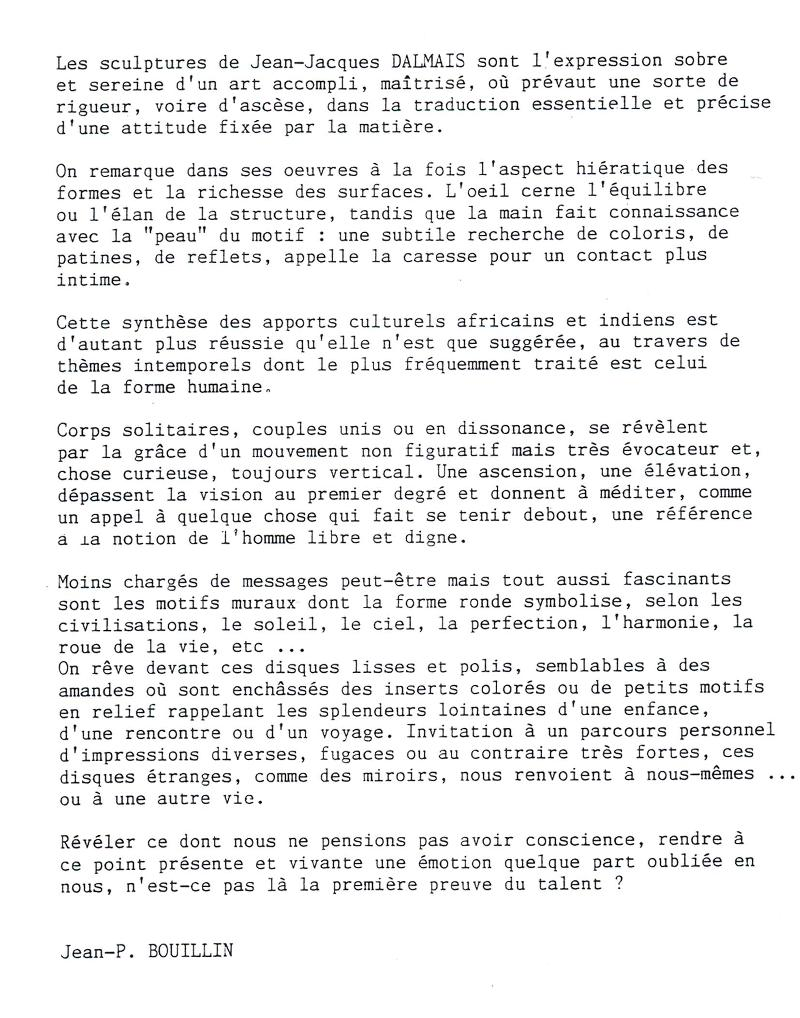
\includegraphics[width=160mm]{texte2.jpg}\\
\caption{ }
\end{center}


\subsection{L'image obtenu apr\`es pr\'etraitement}
\begin{center}
\includegraphics[width=160mm]{thresholded.jpg}\\
\caption{ }
\end{center}


\subsection{Le texte d\'ecoup\'e en blocs}
\begin{center}
\includegraphics[width=160mm]{segmented.jpg}\\
\caption{ }
\end{center}

\pagebreak

\subsection{Le fichier XML que l'on sort} % (fold)
\label{sub:le_fichier_xml_que_l_on_sort}
\begin{lstlisting}
<p x[57,769] y[51,135]>
	<l x[57,726] y[51,71]>
		<w x[57,86] y[56,69]>
			<c x[57,65] y[51,71] />
			<c x[68,75] y[51,71] />
			<c x[78,86] y[51,71] />
		</w>
		<w x[100,205] y[56,71]>
			<c x[100,108] y[51,71] />
			<c x[111,119] y[51,71] />
			<c x[123,130] y[51,71] />
			<c x[133,140] y[51,71] />
			<c x[145,151] y[51,71] />
			<c x[155,162] y[51,71] />
			<c x[165,173] y[51,71] />
			<c x[176,184] y[51,71] />
			<c x[187,194] y[51,71] />
			<c x[197,205] y[51,71] />
		</w>
		<w x[219,238] y[55,67]>
			<c x[219,227] y[51,71] />
			<c x[230,238] y[51,71] />
		</w>
.
.
.
		<w x[539,600] y[876,889]>
			<c x[539,545] y[831,894] />
			<c x[548,557] y[831,894] />
			<c x[560,567] y[831,894] />
			<c x[571,578] y[831,894] />
			<c x[582,590] y[831,894] />
			<c x[594,600] y[831,894] />
		</w>
		<w x[616,621] y[875,883]>
			<c x[616,621] y[831,894] />
		</w>
	</l>
</p>
<p x[61,232] y[943,958]>
	<l x[61,232] y[943,958]>
		<w x[61,102] y[945,958]>
			<c x[61,70] y[943,958] />
			<c x[72,80] y[943,958] />
			<c x[83,91] y[943,958] />
			<c x[94,102] y[943,958] />
		</w>
		<w x[117,132] y[944,957]>
			<c x[117,124] y[943,958] />
			<c x[130,132] y[943,958] />
		</w>
		<w x[149,232] y[943,956]>
			<c x[149,157] y[943,958] />
			<c x[158,167] y[943,958] />
			<c x[170,178] y[943,958] />
			<c x[181,188] y[943,958] />
			<c x[191,200] y[943,958] />
			<c x[202,211] y[943,958] />
			<c x[213,220] y[943,958] />
			<c x[224,232] y[943,958] />
			<c x[224,226] y[943,958] />
		</w>
	</l>
</p>	
\end{lstlisting}
% subsection le_fichier_xml_que_l_on_sort (end)
% section pr'etraitement (end)

\end{document}
